\documentclass[12pt]{beamer}
\newenvironment{ConCodigo}[1]
  {\begin{frame}[fragile,environment=ConCodigo]{#1}}
  {\end{frame}}
\graphicspath{{Imagenes/}{../Imagenes/}}
\usepackage[utf8]{inputenc}
\usepackage[spanish]{babel}
\usepackage{hyperref}
\usepackage{etex}
\reserveinserts{28}
\usepackage{amsmath}
\usepackage{amsthm}
\usepackage{mathtools}
\usepackage{multicol}
\usepackage{multirow}
\usepackage{tabulary}
%\usepackage{tabularx}
\usepackage{booktabs}
\usepackage{nccmath}
\usepackage{biblatex}
\usepackage{epstopdf}
\usepackage{graphicx}
\usepackage{siunitx}
\sisetup{scientific-notation=true}
%\usepackage{fontspec}
\usepackage{lmodern}
\usepackage{float}
\usepackage[format=hang, font=footnotesize, labelformat=parens]{caption}
\usepackage[autostyle,spanish=mexican]{csquotes}
\usepackage{standalone}
\usepackage{tikz}
\usepackage[siunitx]{circuitikz}
\usetikzlibrary{arrows,patterns,shapes}
\usetikzlibrary{decorations.markings}
\usetikzlibrary{arrows}
\usepackage{color}
%\usepackage{beton}
%\usepackage{euler}
%\usepackage[T1]{fontenc}
\usepackage[sfdefault]{roboto}  %% Option 'sfdefault' only if the base font of the document is to be sans serif
\usepackage[T1]{fontenc}
\renewcommand*\familydefault{\sfdefault}
\DeclareGraphicsExtensions{.pdf,.png,.jpg}
\usepackage{hyperref}
\renewcommand {\arraystretch}{1.5}
\newcommand{\python}{\texttt{python}}
\usefonttheme[onlymath]{serif}
\setbeamertemplate{navigation symbols}{}
\usetikzlibrary{patterns}
\usetikzlibrary{decorations.markings}
\tikzstyle{every picture}+=[remember picture,baseline]
%\tikzstyle{every node}+=[inner sep=0pt,anchor=base,
%minimum width=2.2cm,align=center,text depth=.15ex,outer sep=1.5pt]
%\tikzstyle{every path}+=[thick, rounded corners]
\setbeamertemplate{caption}[numbered]
\newcommand{\ptm}{\fontfamily{ptm}\selectfont}
%Se usa la plantilla Warsaw modificada con spruce
\mode<presentation>
{
  \usetheme{Warsaw}
  \setbeamertemplate{headline}{}
  \useoutertheme{default}
  \usecolortheme{beaver}
  \setbeamercovered{invisible}
}
\AtBeginSection[]
{
\begin{frame}<beamer>{Contenido}
\normalfont\mdseries
\tableofcontents[currentsection]
\end{frame}
}

\usepackage{listings}
\lstset{ %
language=Python,                % choose the language of the code
basicstyle=\small,       % the size of the fonts that are used for the code
numbers=left,                   % where to put the line-numbers
numberstyle=\small,      % the size of the fonts that are used for the line-numbers
stepnumber=1,                   % the step between two line-numbers. If it is 1 each line will be numbered
numbersep=5pt,                  % how far the line-numbers are from the code
backgroundcolor=\color{white},  % choose the background color. You must add \usepackage{color}
showspaces=false,               % show spaces adding particular underscores
showstringspaces=false,         % underline spaces within strings
showtabs=false,                 % show tabs within strings adding particular underscores
frame=single,   		% adds a frame around the code
tabsize=2,  		% sets default tabsize to 2 spaces
captionpos=b,   		% sets the caption-position to bottom
breaklines=true,    	% sets automatic line breaking
breakatwhitespace=false,    % sets if automatic breaks should only happen at whitespace
escapeinside={\%},          % if you want to add a comment within your code
stringstyle =\color{magenta},
keywordstyle = \color{blue},
commentstyle = \color{green},
identifierstyle = \color{red}
}
\usepackage{siunitx}
\usepackage[american,cuteinductors,smartlabels]{circuitikz}
\usetikzlibrary{calc}
\title{Ecuaciones diferenciales ordinarias}
\subtitle{Curso de Física Computacional}
\author[]{M. en C. Gustavo Contreras Mayén}
\begin{document}
\maketitle
\fontsize{14}{14}\selectfont
\spanishdecimal{.}
\begin{frame}{Contenido}
\tableofcontents[pausesections]
\end{frame}
\section{Métodos de Runge-Kutta}
\begin{frame}
El principal inconveniente del método de series de Taylor es que requiere que se aplique de manera repetida la diferenciación a las variables dependientes.
\\
\medskip
Evaluar estas expresiones puede llegar a ser una tarea muy extendida y son, por tanto, propensas a errores y tediosas de calcular. Adicionalmente, existe el trabajo extra de codificar cada una de los derivadas.
\end{frame}
\begin{frame}
El objetivo de los métodos de Runge-Kutta (RK) es eliminar la necesidad de la diferenciación repetida de las ecuaciones diferenciales. 
\\
\medskip
Dado que la diferenciación repetida no está implicada en la fórmula de integración en serie de Taylor de primer orden
\[ \mathbf{y}(x+h) = \mathbf{y}(x) + \mathbf{y}'(x) h = \mathbf{y}(x) + \mathbf{F}(x,\mathbf{y}) h \]
Se considera como el método Runge-Kutta de primer orden (RK1), también llamado, \emph{método de Euler}. Como el error de truncamiento es bastante, no se usa en la práctica común.
\end{frame}
\begin{frame}
\frametitle{Representación del método de Euler}
\begin{center}
\begin{tikzpicture}[scale=0.8, font=\small]
	\draw (0,0) -- (8,0);
	\draw (0,0) -- (0,4);
	\draw (-0.3,4.3) node {$y'(x)$};
	\draw (8.3,-0.3) node {$x$};
	\draw [pattern=north east lines] (2.5,0) rectangle (5.5,2);
	\draw (2.5,-0.5) node {$x$};
	\draw (5.5,-0.5) node {$x+h$};
	\draw (1.5,1) node {$f(x,y)$};
	\draw (2.5,2) circle (0.05);
	\draw [blue, thick](2.3,1.6) .. controls(3,3) and (4.5,4) .. (6,4.5);
	\draw [dashed] (5.5,0) -- (5.5,4.3);
	\draw (5.5,4.3) circle (0.05);
	\draw [black] (4,1) circle (0.05);
	\draw (4,1) -- (7,1.4);
	\draw [align=center](7.2,1.4) node {Fórmula \\ de Euler};
	\draw [black] (4.3,3) circle (0.05);
	\draw (4.3,3) -- (7,3.5);
	\draw (7.5,3.5) node {Error};
\end{tikzpicture}
\end{center}
Para simplificar, consideremos que tenemos una sola variable $y$, y que la ecuación diferencial es $y'=f(x,y)$.
\end{frame}
\begin{frame}
El cambio en la solución $y$ entre $x$ y $x+h$ es
\[ y(x+h) - y(h) = \int_{x}^{x+h} y' dx = \int_{x}^{x+h} f(x,y) dx \]
que es el área debajo de la gráfica de $y'(x)$.
\\
\medskip
La fórmula de Euler aproxima ésta área con el área del rectángulo sombreado. El área entre el rectángulo sombreado y la gráfica representa el error debido al truncamiento.
\\
\medskip
Se revisa claramente que el error de truncamiento es proporcional a la pendiente de la gráfica, esto es, proporcional a $y'(x)$
\end{frame}
\section{Método RK2}
\begin{frame}
\frametitle{Método de Runge-Kutta de segundo orden}
Para obtener el método RK2, suponemos una fórmula de integración del tipo
\fontsize{12}{12}\selectfont
\[ \mathbf{y}(x+h) = \mathbf{y}(x) + c_{0} \mathbf{F}(x,\mathbf{y})h + c_{1} \mathbf{F}[x+ph, \mathbf{y}+qh \mathbf{F}(x,\mathbf{y})] h \]
\fontsize{14}{14}\selectfont
e intentamos encontrar los parámetros $c_{0}$, $c_{1}$, $p$ y $q$ de tal forma que se parezca a la serie de Taylor
\[ \begin{split}
\mathbf{y}(x+h) &= \mathbf{y}(x) + \mathbf{y}'(x) h + \dfrac{1}{2!}\mathbf{y}''(x) h^{2} + O(h^{3}) \\
&= \mathbf{y}(x) + \mathbf{F}(x,\mathbf{y}) h + \dfrac{1}{2}\mathbf{F}'(x,\mathbf{y}) h^{2} + O(h^{3})
\end{split} \]
\end{frame}
\begin{frame}
Notemos que
\[ \mathbf{F}'(x,\mathbf{y}) = \dfrac{\partial \mathbf{F}}{\partial x} + \sum_{i=0}^{n-1} \dfrac{\partial \mathbf{F}}{\partial \mathbf{y}_{i}} \mathbf{y}'_{i} = \dfrac{\partial \mathbf{F}}{\partial x} + \sum_{i=0}^{n-1} \dfrac{\partial \mathbf{F}}{\partial \mathbf{y}_{i}} F_{i}(x,\mathbf{y})\]
donde $n$ es el número de 1-EDO.
\end{frame}
\begin{frame}
Entonces podemos escribir para $\mathbf{y}(x+h)$ como
\[ \begin{split}
\mathbf{y}(x+h) &= \mathbf{y}(x) + \mathbf{F}(x,\mathbf{y})h + \\
&= \dfrac{1}{2} \left( \dfrac{\partial \mathbf{F}}{\partial x} + \sum_{i=0}^{n-1} \dfrac{\partial \mathbf{F}}{\partial \mathbf{y}_{i}} F_{i}(x,\mathbf{y}) \right) h^{2} + O(h^{3})
\end{split} \]
\end{frame}
\begin{frame}
Regresando a la ecuación inicial, re-escribimos el último término mediante una serie de Taylor en varias variables:
\[ \begin{split}
 \mathbf{F}[x+ph, \mathbf{y}+qh \mathbf{F}(x,\mathbf{y})] &= \mathbf{F}(x,\mathbf{y}) + \dfrac{\partial \mathbf{F}}{\partial x} ph + \\
 &+ qh \sum_{i=1}^{n-1} \dfrac{\partial \mathbf{F}}{\partial y_{i}} F_{i}(x,\mathbf{y}) + O(h^{2}) 
\end{split} \]
\end{frame}
\begin{frame}
Por lo que la ecuación inicial, toma la forma:
\[  \begin{split}
\mathbf{y}(x+h) &= \mathbf{y}(x) + (c_{0}+c_{1})\mathbf{F}(x,\mathbf{y})h + \\
&+ c_{1} \left[ \dfrac{\partial \mathbf{F}}{\partial x} ph + qh \sum_{i=1}^{n-1} \dfrac{\partial \mathbf{F}}{\partial y_{i}} F_{i}(x,\mathbf{y}) \right] h + O(h^{3}) 
\end{split} \]
Para que las expresiones sean idénticas, se necesita que:
\[ c_{0}+c_{1}= 1 \hspace{1cm} c_{1}p = \dfrac{1}{2} \hspace{1cm} c_{1}q = \dfrac{1}{2}\]
\end{frame}
\begin{frame}
El conjunto anterior representa un sistema de tres ecuaciones y cuatro incógnitas, por lo que se asigna un valor a cualquiera de ellas.
\\
\medskip
Las opciones más comunes y sus nombres para los métodos son los siguientes:
\\
\bigskip
\begin{tabular}{l | l | l | l | l}
$c_{0}=0$ & $c_{1}=1$ & $p=\frac{1}{2}$ & $q=\frac{1}{2}$ & Euler modificado \\ \hline
$c_{0}=\frac{1}{2}$ & $c_{1}=\frac{1}{2}$ & $p=1$ & $q=1$ & Heun \\ \hline
$c_{0}=\frac{1}{3}$ & $c_{1}=\frac{2}{3}$ & $p=\frac{3}{4}$ & $q=\frac{3}{4}$ & Ralston
\end{tabular}
\\
\medskip
Todas estas fórmulas son del tipo RK2, ninguna tiene una superioridad numérica con respecto a las otras.
\end{frame}
\subsection{Método de Euler modificado}
\begin{frame}
\frametitle{Método de Euler modificado}
Sustituimos los valores de los parámetros en la ecuación general para obtener:
\[ \mathbf{y}(x+h) = \mathbf{y}(x) + \mathbf{F} \left[  x + \dfrac{h}{2}, \mathbf{y} + \dfrac{h}{2} \mathbf{F}(x,\mathbf{y}) \right] h\]
Esta fórmula de integración puede evaluarse convenientemente, siguiendo la siguiente secuencia de operaciones:
\begin{eqnarray*}
\mathbf{K}_{0} &=& h \mathbf{F}(x,\mathbf{y}) \\
\mathbf{K}_{1} &=& h \mathbf{F} \left( x+\dfrac{h}{2},\mathbf{y}+\dfrac{1}{2} \mathbf{K}_{0} \right) \\
\mathbf{y}(x+h) &=& \mathbf{y}(x) + \mathbf{K}_{1}
\end{eqnarray*}
\end{frame}
\begin{frame}
\frametitle{Representación del método de Euler modificado}
\begin{center}
\begin{tikzpicture}[scale=0.8, font=\small]
	\draw (0,0) -- (8,0);
	\draw (0,0) -- (0,4);
	\draw (-0.3,4.3) node {$y'(x)$};
	\draw (8.3,-0.3) node {$x$};
	\draw (2.5,0) rectangle (5.5,3.5);
	\draw (2.5,-0.5) node {$x$};
	\draw (5.5,-0.5) node {$x+h$};
	\draw (1.5,1) node {$f(x,y)$};
	\draw (2.5,2) circle (0.05);
	\draw (2.5,2) -- (1.3,2);
	\draw [->] (1.5,1.3) -- (1.5,2);
	\draw [->] (1.5,0.7) -- (1.5,0);
	\draw [blue, thick](2.3,1.6) .. controls(3,3) and (4.5,4) .. (6,4.5);
	\draw [dashed] (5.5,0) -- (5.5,4.3);
	\draw (5.5,4.3) circle (0.05);
	\draw [dashed] (4,0) -- (4,3.5);
	\draw [<->] (2.5,1) --  node [above=0.2] {$\frac{h}{2}$}(4,1);
	\draw [<->] (4,1) --  node [above=0.2] {$\frac{h}{2}$}(5.5,1);
	\draw (5.5,3.5) -- (7,3.5);
	\draw (8,1.8) node {$f(x+h/2, y+K_{0}/2)$};
	\draw [->] (6.5,2.1) -- (6.5,3.5);
	\draw [->] (6.5,1.5) -- (6.5,0);	
\end{tikzpicture}
\end{center}
Representación gráfica del método de Euler modificado para una EDO $y'=f(x,y)$.
\end{frame}
\begin{frame}
El valor de $\mathbf{K}_{0}= h \mathbf{F}(x,\mathbf{y})$ devuelve un estimado de $y$ en el punto central para la fórmula de Euler
\[ y(x+\frac{h}{2}) = y(x) + f(x,y) \frac{h}{2} = y(x) + \frac{K_{0}}{2}\]
La segunda ecuación $\mathbf{K}_{1}$, aproxima el área del bloque por el área $K_{1}$ del rectángulo. El error es proporcional a la curvatura $y'''$ de la gráfica.
\end{frame}
\begin{frame}
\frametitle{Ejemplo}
Utiliza RK2 para integrar la siguiente EDO:
\[ y' = \sin y \hspace{1.5cm} y(0) = 1\]
de $x=0$ a $x=0.5$ en pasos de $h=0.1$
\end{frame}
\begin{frame}
\frametitle{Solución}
Del problema tenemos que:
\[ F(x,y) = \sin y\]
por lo que las fórmular canónicas de integración son
\begin{eqnarray*}
K_{0} &=& h F(x,y) = 0.1 \sin y \\
K_{1} &=& h F \left( x + \dfrac{h}{2}, y + \dfrac{1}{2} K_{0} \right) = 0.1 \sin \left(  y + \dfrac{1}{2} K_{0}\right) \\
y(x+h) &=& y(x) + K_{1}
\end{eqnarray*}
\end{frame}
\begin{frame}
Como $y(0) = 1$, podemos integrar
\begin{eqnarray*}
K_{0} &=& 0.1 \sin (1.0000) = 0.0841 \\
K_{1} &=& 0.1 \sin \left( 1.0000 + \dfrac{0.0841}{2} \right)  = 0.0863 \\
y(0.1) &=& 1.0 + 0.0863 = 1.0863
\end{eqnarray*}
\pause
\begin{eqnarray*}
K_{0} &=& 0.1 \sin (1.0863) = 0.0885 \\
K_{1} &=& 0.1 \sin \left( 1.0.0863 + \dfrac{0.0885}{2} \right)  = 0.0905 \\
y(0.2) &=& 1.0863 + 0.0905 = 1.1768
\end{eqnarray*}
y así, sucesivamente.
\end{frame}
\begin{frame}
A manera de resumen, las cuentas se presentan en la siguiente tabla:
\begin{center}
\begin{tabular}{c | c | c | c |}
$x$ & $y$ & $K_{0}$ & $K_{1}$ \\ 
\hline
\hline
0.0 & 1.0000 & 0.0841 & 0.0863 \\ \hline
0.1 & 1.0863 & 0.0885 & 0.0905 \\ \hline
0.2 & 1.1768 & 0.0923 & 0.0940 \\ \hline
0.3 & 1.2708 & 0.0955 & 0.0968 \\ \hline
0.4 & 1.3676 & 0.0979 & 0.0988 \\ \hline
0.5 & 1.4664 & & \\ \hline
\end{tabular}
\end{center}
\end{frame}
\begin{frame}
La solución exacta (que podrían demostrar que cumple) es:
\[ x(y) = ln(\csc y - \cot y) + 0.604582 \]
que devuelve en $x(1.4664) = 0.5000)$
\\
\bigskip
Sin embargo, es poco probable que esta precisión se mantenga mientras continuemos integrando, dado que los errores (tanto de truncamiento como de redondeo) se van acumulando, si tenemos un rango amplio de integración, se requiere de mejores fórmulas de integración.
\end{frame}
\section{Método RK4}
\begin{frame}
\frametitle{Método de Runge-Kutta de cuarto orden}
El método de RK4 se obtiene de la serie de Taylor, de la misma forma como se obtuvo RK2; considerando que la derivación es un proceso largo y no tan instructivo, por lo que lo omitiremos.
\\
\medskip
La expresión final de la fórmula de integración también depende de la elección de los parámetros, es decir, no hay una única fórmula para RK4.
\end{frame}
\begin{frame}
La expresión más popular se le conoce como método RK4, que requiere de las siguientes operaciones:
\begin{eqnarray*}
K_{0} &=& h \mathbf{F}(x,\mathbf{y}) \\
K_{1} &=& h \mathbf{F}(x +\dfrac{h}{2},\mathbf{y} + \dfrac{\mathbf{K}_{0}}{2}) \\
K_{2} &=& h \mathbf{F}(x +\dfrac{h}{2},\mathbf{y} + \dfrac{\mathbf{K}_{1}}{2}) \\
K_{3} &=& h \mathbf{F}(x +h, \mathbf{y} + \mathbf{K}_{2}) \\
\mathbf{y}(x+h) &=& \mathbf{y}(x) + \dfrac{1}{6} (\mathbf{K}_{0} + 2 \mathbf{K}_{1} + 2 \mathbf{K}_{2} + \mathbf{K}_{3})
\end{eqnarray*}
\end{frame}
\begin{frame}
El principal inconveniente de este método es que no se presta para una estimación del error de truncamiento. Por lo tanto, tenemos que ''adivinar'' el tamaño del paso de integración $h$, o determinarlo por ensayo y error.
\\
\medskip
En contraste, los llamados métodos adaptativos pueden evaluar el error de truncamiento en cada paso de integración y ajustar el valor de $h$ en consecuencia, pero con un gran costo, computacionalmente hablando.
\end{frame}
\subsection{Algoritmo RK4}
\begin{frame}
\frametitle{Algoritmo RK4}
La función \texttt{integra} en este módulo, implementa el método RK4. El usuario deberá de proporcionar en \texttt{integra} la función \texttt{F(x,y)} que define el conjunto de 1-EDO $\mathbf{y}' = \mathbf{F}(x,\mathbf{y})$. 
\end{frame}
\begin{frame}[fragile]
\begin{lstlisting}
def integra(F,x,y,xAlto,h):
    
    def rk_4(F,x,y,h):
        K0 = h*F(x,y)
        K1 = h*F(x + h/2.0, y + K0/2.0)
        K2 = h*F(x + h/2.0, y + K1/2.0)
        K3 = h*F(x + h, y + K2)
        return (K0 + 2.0*K1 + 2.0*K2 + K3) / 6.0
    
    X = []
    Y = []
    X.append(x)
    Y.append(y)
\end{lstlisting}
\end{frame}
\begin{frame}[fragile]
\begin{lstlisting}
    while x < xAlto:
        h = min(h, xAlto - x)
        y = y + rk_4(F,x,y,h)
        x = x + h
        X.append(x)
        Y.append(y)
    
    return array(X), array(Y)
\end{lstlisting}
\end{frame}
\begin{frame}
\frametitle{Ejemplo}
Resolver
\[ y'' = -0.1 y' - x \hspace{1.5cm} y(0) = 0 \hspace{1cm} y'(0)=1\]
de $x=0$ a $x=2$ con incrementos de $h=0.25$ mediante RK4.
\end{frame}
\begin{frame}
Usando la notación $y_{0}= y$ junto con $y_{1} = y'$, podemos escribir un conjunto de 1-EDO como
\begin{equation*} 
\mathbf{y}' = \mathbf{F}(x,\mathbf{y}) =
\begin{bmatrix}
y'_{0} \\
y'_{1}
\end{bmatrix} = 
\begin{bmatrix}
y_{1} \\
-0.1 y_{1} - x
\end{bmatrix}
\end{equation*}
\end{frame}
\begin{frame}[fragile]
\frametitle{Código completo}
\begin{lstlisting}
def F(x,y):
    F = zeros((2), dtype='float64')
    F[0] = y[1]
    F[1] = -0.1 * y[1]
    return F

x=0.0
xAlto=2.0
y = array([0.0,1.0])
h=0.25
freq=1

X,Y = integra(F,x,y,xAlto,h)
imprimeSoln(X,Y,freq)
\end{lstlisting}
\end{frame}
\begin{frame}
\frametitle{Resultado}
\begin{center}
\begin{tabular}{c | c | c }
x & y[0] & y[1] \\ \hline 
   0.0000e+00 & 0.0000e+00 & 1.0000e+00 \\ \hline
   2.5000e-01 & 2.4690e-01 & 9.7531e-01 \\ \hline
   5.0000e-01 & 4.8771e-01 & 9.5123e-01 \\ \hline
   7.5000e-01 & 7.2257e-01 & 9.2774e-01 \\ \hline
   1.0000e+00 & 9.5163e-01 & 9.0484e-01 \\ \hline
   1.2500e+00 & 1.1750e+00 & 8.8250e-01 \\ \hline
   1.5000e+00 & 1.3929e+00 & 8.6071e-01 \\ \hline
   1.7500e+00 & 1.6054e+00 & 8.3946e-01 \\ \hline
   2.0000e+00 & 1.8127e+00 & 8.1873e-01
\end{tabular}
\end{center}
\end{frame}
\begin{frame}
\frametitle{Ejercicio 2}
Usa RK4 para integrar
\[ y' = 3y - 4 e^{-x} \hspace{1.5cm} y(0)=1 \]
desde $x=0$ hasta $x=10$ en pasos de $h=0.1$. Comparar el resultado con la solución analítica $y=\exp(-x)$
\\
\bigskip
Usaremos el programa anterior. Recordemos que \texttt{rk\_4} supone que $y$ es un arreglo, por lo que debemos de especificar la condición inicial como $y=\text{array}([1.0])$ y no $y=1.0$
\end{frame}
\begin{frame}[fragile]
\begin{lstlisting}
def F(x,y):
    F = zeros((1), dtype='float64')
    F[0] = 3.0 * y[0] - 4.0 * exp(-x)
    return F


x = 0.0
xAlto = 10.0
y = array([1.0])
h = 0.1
freq = 20

X,Y = integra(F,x,y,xAlto,h)
imprimeSoln(X,Y,freq)
\end{lstlisting}
\end{frame}
\begin{frame}
\frametitle{Resultado}
\begin{center}
\begin{tabular}{c | c }
x  &  y[0] \\ \hline 
   0.0000e+00 & 1.0000e+00 \\ \hline
   2.0000e+00 & 1.3250e-01 \\ \hline
   4.0000e+00 & -1.1237e+00 \\ \hline
   6.0000e+00 & -4.6056e+02 \\ \hline
   8.0000e+00 & -1.8575e+05 \\ \hline
   1.0000e+01 & -7.4912e+07
\end{tabular}
\end{center}
Pero ¿es correcto esto?
\end{frame}
\begin{frame}
De acuerdo a la solución numérica, $y$ debería de acercarse a cero conforme se incrementa $x$, pero el resultado nos muestra lo contrario: después de un incremento inicial, la magnitud de $y$ se incrementa súbitamente.
\\
\bigskip
Podemos explicar esto mirando de cerca la solución analítica.
\end{frame}
\begin{frame}
La solución general de la EDO dada es
\[ y = C e^{3x} + e^{-x} \]
que puede verificarse por sustitución.
\\
\medskip
La condición inicial $y(0)=1$ hace que $C=0$, que para la solución del problema, es precisamente $y=exp(-x)$.
\end{frame}
\begin{frame}
El problema en la solución numérica es el término dominante $Ce^{3x}$
\\
\medskip
Supongamos que la condición inicial tiene un pequeño error $\epsilon$, por lo que tenemos $y(0)=1+\epsilon$. Esto cambia la solución analítica por
\[ y = \epsilon e^{3x} + e^{-x} \]
\end{frame}
\begin{frame}
\[ y = \epsilon e^{3x} + e^{-x} \]
Vemos que el término que contiene el error $\epsilon$, se hace dominante conforme $x$ aumenta. Dado que los errores son inherentes a las soluciones numéricas, tenemos el mismo efecto para cambios pequeños en las condiciones iniciales, por lo que concluimos que nuestra solución numérica es víctima de la \emph{inestabilidad numérica}, debida a la sensibilidad de la solución a las condiciones iniciales.
\end{frame}
\begin{frame}
\frametitle{Ejercicio más elaborado}
\begin{center}
\begin{tikzpicture}[font=\small]
	\draw (2,2) circle (2cm);
	\draw [dashed] (-0.4,2) -- (5,2);
	\draw [->] (2,2) -- node [midway, fill=white] {$R_{t}$} (1.8,4);
	\draw (5,2) circle (0.05);
	\draw (5.2,1.8) node {H}; 
	\draw [->] (5,2) -- node [near end, right] {$v_{0}$}(5,2.5);
	\draw [->] (2,2) -- node [midway, above] {$r$} (4,3.6);
	\draw (2.7,2) arc (0:45:5.9mm) node [right] {$\theta$};
	\draw [dashed] (5,2) arc (0:95:1.8);
\end{tikzpicture}
\end{center}
Un satélite se lanza desde una altitud $H=772$ km sobre el nivel del mar, con una velocidad inicial $v_{0}=6700$ $m/s$ en la dirección que se muestra.
\end{frame}
\begin{frame}
El conjunto de EDO que describen el movimiento del satélite son:
\[ \ddot{r} = r  \dot{\theta}^{2} - \dfrac{G M_{t}}{r^{2}}  \hspace{2cm} \ddot{\theta} = - \dfrac{2 \dot{r}\dot{\theta}}{r}\]
donde $r$ y $\theta$ son las coordenadas polares del satélite.
\\
\medskip
Las constantes involucradas en las expresiones, son:
\begin{eqnarray*}
G &=& 6.672 \times 10^{-11} \mbox{m}^{3} \mbox{kg}^{-1} \mbox{s}^{2} \\
M_{t} &=& 5.9742 \times 10^{24} \mbox{kg, Masa de la Tierra} \\
R_{e} &=& 6378.14 \mbox{km, radio de la Tierra al nivel del mar} 
\end{eqnarray*}
\end{frame}
\begin{frame}
\frametitle{Problema a resolver}
\begin{enumerate}
\item Obtén el conjunto de 1-EDO y las condiciones iniciales del problema, de la forma $\dot{\mathbf{y}} = \mathbf{F}(x,\mathbf{y})$, $\mathbf{y}(0) = \mathbf{b}$.
\item Con RK4 integra las 1-EDO en el tiempo en que se lanza el satélite y choca en su regreso a la Tierra.
\item Calcula el lugar del impacto, con $\theta$.
\end{enumerate}
\end{frame}
\begin{frame}
\frametitle{Inciso 1)}
Tenemos que
\[ \begin{split} G M_{t} &= (6.672 \times 10^{-11}) (5.9742 \times 10^{24})  = \\
 &= 3.9860 \times 10^{14} \mbox{m}^{3} \mbox{s}^{2} \end{split} \]
Ahora hacemos
\[ \mathbf{y} = \begin{bmatrix}
y_{0} \\
y_{1} \\
y_{2} \\
y_{3}
\end{bmatrix} =
\begin{bmatrix}
r \\
\dot{r} \\
\theta \\
\dot{\theta}
\end{bmatrix}
\]
\end{frame}
\begin{frame}
Por lo que el conjunto equivalente de 1-EDO, resulta ser
\[ \dot{\mathbf{y}} = \begin{bmatrix}
\dot{y}_{0} \\
\dot{y}_{1} \\
\dot{y}_{2} \\
\dot{y}_{3}
\end{bmatrix} =
\begin{bmatrix}
y_{1} \\
y_{0} y_{3}^{2} - 3.9860 \times 10^{14}/y_{0}^{2} \\
y_{3} \\
-2 y_{1} y_{3} / y_{0}
\end{bmatrix} \]
\end{frame}
\begin{frame}
Las condiciones iniciales resultan
\fontsize{12}{12}\selectfont
\begin{eqnarray*}
r(0) &=& R_{t} + H = (6378.14+772) \times 10^{3} = 7.15014 \times 10^{6} \mbox{ m} \\
\dot{r}(0) &=& 0 \\
\theta(0) &=& 0 \\
\dot{\theta}(0) &=& \dfrac{v_{0}}{r(0)} = \dfrac{6700}{7.15014 \times 10^{6}} = 0.937045 \times 10^{-3} \mbox{ rad/s}
\end{eqnarray*}
\fontsize{14}{14}\selectfont
Por tanto
\[ \mathbf{y}(0) = 
\begin{bmatrix}
7.15014 \times 10^{6} \\
0 \\
0 \\
0.937045 \times 10^{3}
\end{bmatrix}
\]
\end{frame}
\begin{frame}
\frametitle{Inciso 2)}
Usaremos lo que ya hemos construido con el programa \texttt{integra}, para continuar con la notación, la variable independiente $t$, la escribimos como $x$.
\\
\medskip
El período de integración, es decir, el valor de \texttt{xAlto} cuando el satélite choca con la Tierra, hay que estimarlo tentativamente.
\end{frame}
\begin{frame}[fragile]
\begin{lstlisting}
def F(x,y):
    F = zeros((4), dtype='float64')
    F[0] = y[1]
    F[1] = y[0]*(y[3]**2) - 3.9860e14 / (y[0]**2)
    F[2] = y[3]
    F[3] = -2.0*y[1]*y[3]/y[0]
    return F

x = 0.0
xAlto =
y = array([7.1514e6, 0.0 , 0.0, 0.937045e-3])
h = 50.0
freq = 2
X,Y = integra(F,x,y,xAlto,h)
imprimeSoln(X,Y,freq)
\end{lstlisting}
\end{frame}
\begin{frame}
\frametitle{Resultados}
\fontsize{10}{10}\selectfont
\begin{tabular}{c | c | c | c | c}
 x   & y[0] & y[1] & y[2] & y[3] \\ \hline 
   0.0000e+00 & 7.1514e+06 & 0.0000e+00 & 0.0000e+00 & 9.3704e-04 \\ \hline
   1.0000e+02 & 7.1438e+06 & -1.5134e+02 & 9.3771e-02 & 9.3903e-04 \\ \hline
   2.0000e+02 & 7.1212e+06 & -3.0199e+02 & 1.8794e-01 & 9.4502e-04 \\ \hline
   3.0000e+02 & 7.0835e+06 & -4.5121e+02 & 2.8291e-01 & 9.5510e-04 \\ \hline
   4.0000e+02 & 7.0310e+06 & -5.9819e+02 & 3.7910e-01 & 9.6942e-04 \\ \hline
   5.0000e+02 & 6.9639e+06 & -7.4201e+02 & 4.7694e-01 & 9.8817e-04 \\ \hline
   6.0000e+02 & 6.8827e+06 & -8.8159e+02 & 5.7689e-01 & 1.0116e-03 \\ \hline
   7.0000e+02 & 6.7878e+06 & -1.0156e+03 & 6.7944e-01 & 1.0401e-03 \\ \hline
   8.0000e+02 & 6.6798e+06 & -1.1426e+03 & 7.8510e-01 & 1.0740e-03 \\ \hline
   9.0000e+02 & 6.5596e+06 & -1.2605e+03 & 8.9443e-01 & 1.1138e-03 \\ \hline
   1.0000e+03 & 6.4281e+06 & -1.3671e+03 & 1.0081e+00 & 1.1598e-03 \\ \hline
   1.1000e+03 & 6.2866e+06 & -1.4595e+03 & 1.1266e+00 & 1.2126e-03 \\ \hline
   1.2000e+03 & 6.1368e+06 & -1.5343e+03 & 1.2508e+00 & 1.2725e-03
\end{tabular}
\end{frame}
\begin{frame}
El satélite choca con la Tierra cuando $r$ es igual a $R_{t}=6.37814 \times 10^{6}$ m. De los resultados, vemos que esto ocurre entre el tiempo $t= 1000$ y $1100$ segundos.
\\
\medskip
Un valor de $t$ más preciso, lo podemos obtener mediante una interpolación polinomial, pero si no queremos una precisión alta, con una interpolación lineal, bastará.
\\
\medskip
Hacemos $1000 + \Delta t$ el tiempo para el impacto, por lo que escribimos
\[ r(1000 + \Delta t) = R_{t} \]
\end{frame}
\begin{frame}
Desarrollando $r$ con dos términos de la serie de Taylor, tenemos que
\[ \begin{split} 
r(1000) + \dot{r}(1000) \Delta t &= R_{t} \\
6.4250 \times 10^{6} + (-1.3708 \times 10^{3}) \Delta t &= 6378.14 \times 10^{3}
\end{split} \]
que al despejar, 
\[ \Delta t = 34.184 \mbox{ s} \]
Por lo que el tiempo de impacto es $1034.25$ segundos.
\end{frame}
\begin{frame}
\frametitle{Inciso 3)}
La coordenada $\theta$ del impacto, la podemos calcular de una manera similar, para ello desarrollamos dos términos de la serie de Taylor:
\[ \begin{split}
\theta(1000 + \Delta t) &= \theta(1000) + \dot{\theta}(1000)\Delta t \\
 &= 1.0083 + (1.1605 \times 10^{3} )(34.184) \\
 &= 1.0489 \mbox{ rad} = 60.00^{\circ}
\end{split} \]
\end{frame}
\section{Ejercicios}
\begin{frame}
\frametitle{Ejercicio}
Una masa $M = 0.5$ kg se une al extremo inferior de un resorte sin masa. El extremo superior se fija a una pared en reposo. La masa experimenta una resistencia $R = -B dy/dt$ debida al aire, donde $B$ es una constante de amortiguamiento. La ecuación de movimiento es:
\[ M \dfrac{d^{2}}{dt^{2}}y + B \dfrac{d}{dt}y + ky = 0 \hspace{1cm}y(0)=1,y'(0)=0 \]
donde $k=100$ $k/s^{2}$ y $B=10$ $k/s$
\end{frame}
\begin{frame}
\frametitle{Sistema masa-resorte}
\begin{center}
\begin{tikzpicture}
	\tikzstyle{spring}=[thick,decorate,decoration={zigzag,pre length=0.1cm,post
	  length=0.1cm,segment length=6}]
	\draw (0,0) rectangle (1,1) ;
	\draw (0.5,0.5) node {M};
	\draw (0.3,1) -- (0.3,1.2);
	\draw[spring] (0.3,1.2) -- (0.3,2.2);
	\draw (0.3,2.2) -- (0.3,2.4);
	\draw (0.7,1) -- (0.7,1.5);
	\draw (0.5,1.5) -- (0.9,1.5);
	\draw (0.5,1.5) -- (0.5,1.7);
	\draw (0.9,1.5) -- (0.9,1.7);
	\draw (0.6,1.6) --(0.8,1.6);
	\draw (0.7,1.6) -- (0.7,2.4);
	\draw [pattern=north east lines] (-1,2.4) rectangle (2,2.7);
	\draw (1,0) -- (1.9,0);
	\draw [->] (1.8,2.4) -- node [midway, right] {y} (1.8,0);
\end{tikzpicture}
\end{center}
\[ M \dfrac{d^{2}}{dt^{2}}y + B \dfrac{d}{dt}y + ky = 0 \hspace{1cm}y(0)=1,y'(0)=0 \]
donde $k=100$ $k/s^{2}$ y $B=10$ $k/s$.
\\
\medskip
Calcula $y(t)$ para $0<t<2$, con $h=0.001$, ¿qué pasa si $B=0$?
\end{frame}
\begin{frame}
\frametitle{Solución gráfica}
\begin{figure}
	\centering
	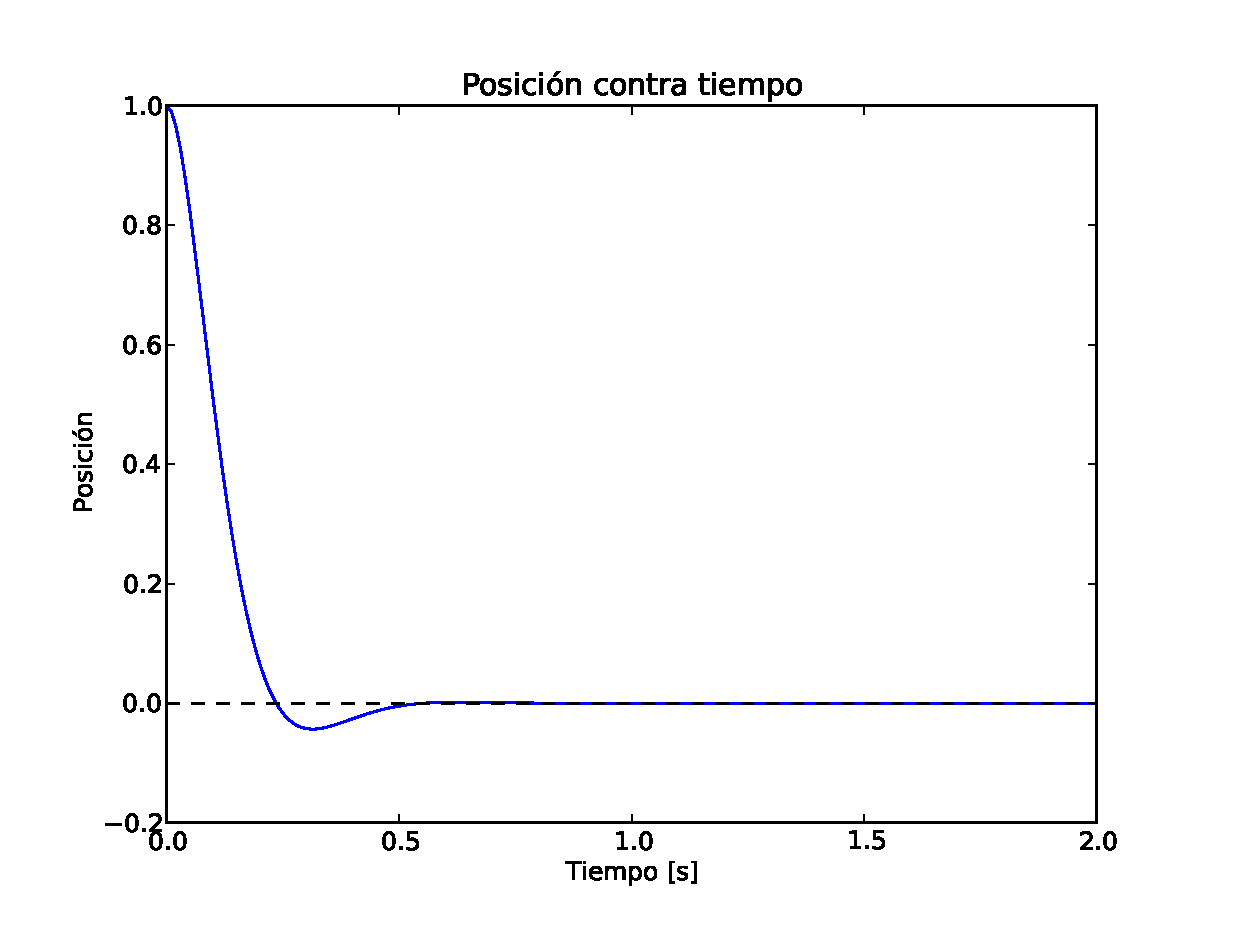
\includegraphics[scale=0.5]{Tema3_2_04_01.eps}<1> 
	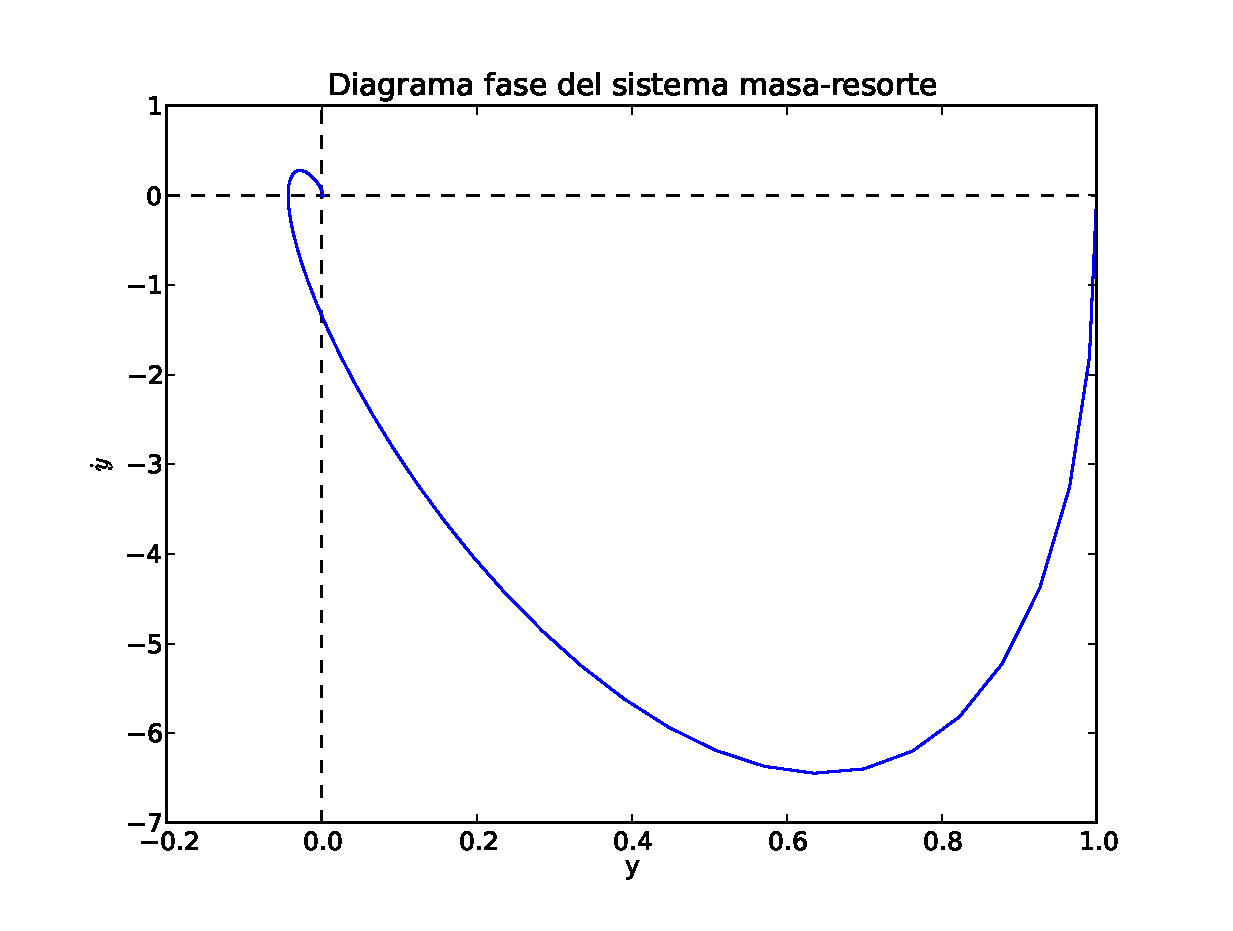
\includegraphics[scale=0.5]{Tema3_2_04_02.eps}<2>
	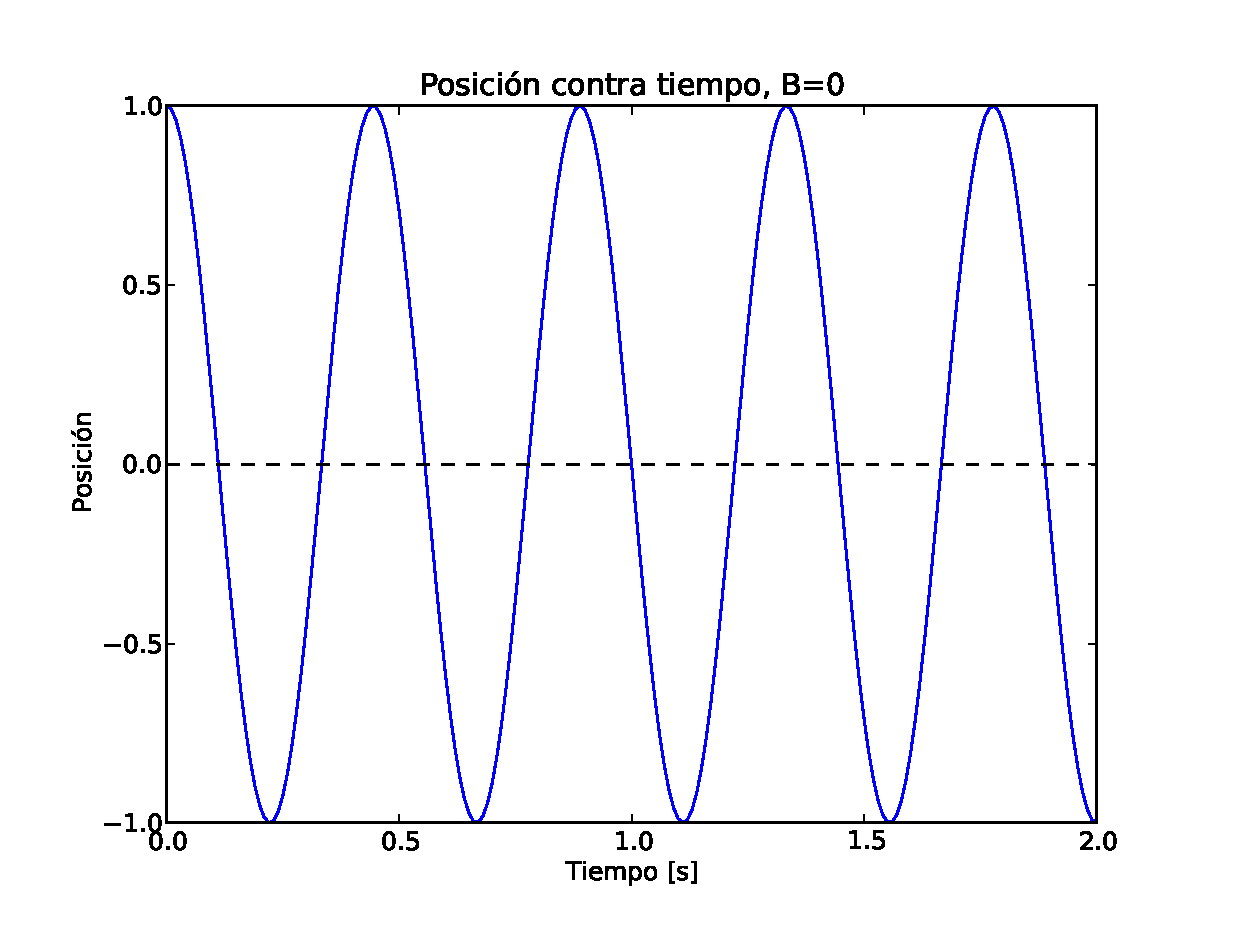
\includegraphics[scale=0.5]{Tema3_2_04_03.eps}<3>
	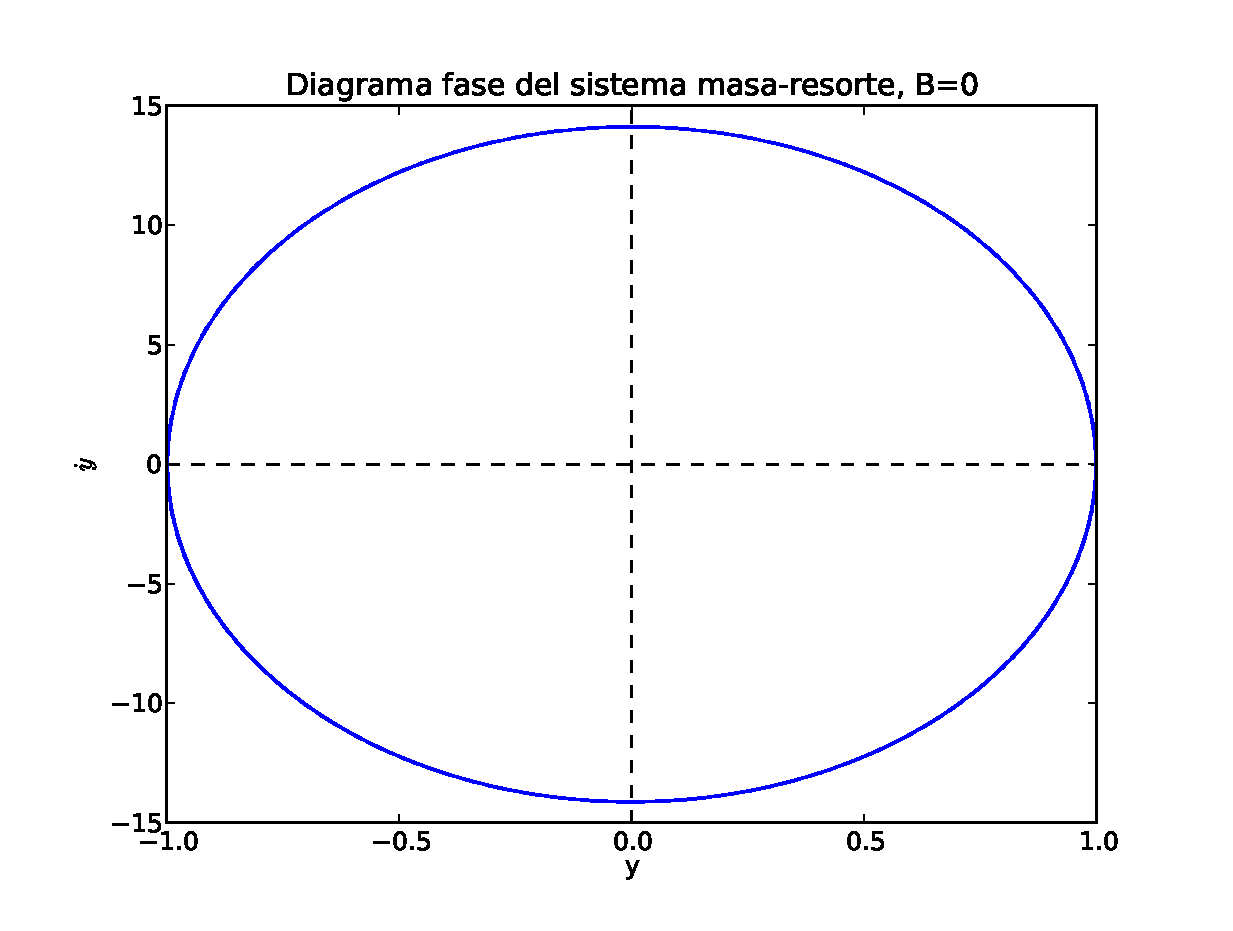
\includegraphics[scale=0.5]{Tema3_2_04_04.eps}<4>
\end{figure}
\end{frame}
\begin{frame}
\frametitle{Ejercicio}
Una pieza metálica con una masa de $0.1$ kg a $200^{\circ}$ C  ($473$ K), se coloca en cierto momento en un cuarto cuya temperatura es $25^{\circ}$ C, en donde la pieza está sujeta al proceso de enfriamiento por convección natural y transferencia de calor por radiación.
\end{frame}
\begin{frame}
Suponemos que la distribución de temperatura es uniforme en la pieza, la ecuación de T vs t es:
\[ \dfrac{dT}{dt} =  \dfrac{A}{(\rho c v)} [ \epsilon \sigma (297^{4} - T^{4})+ h_{c}(297-T)] \]
con $T(0)=473$ donde $T$ es la temperatura en grados Kelvin y las constantes son:
\end{frame}
\begin{frame}
\begin{tabular}{r l}
	$\rho =$  & 300 $\frac{k}{m^{3}}$ -- densidad del metal \\
	$v=$  & 0.001 $m^{3}$ -- volumen del metal \\
	$A=$ & 0.25 $m^{2}$ -- área de la superficie del metal \\
	$c=$ & 900 $\frac{J}{kK}$ -- calor específico del metal \\
	$h_{c}=$ & 30 $\frac{J}{m^{2}K}$ coeficiente de transferencia de calor \\
	$\epsilon=$ & 0.8 -- emisividad del metal \\
	$\sigma=$ & 5.67 $\times 10^{-8}$ $\dfrac{w}{m^{2}K^{2}}$ cte Stefan-Boltzamann
\end{tabular}
Calcular el valor de T para el intervalo $0 < t < 200$ segundos, usa $h=0.25$
\end{frame}
\begin{frame}
\frametitle{Solución gráfica}
\begin{figure}
	\centering
	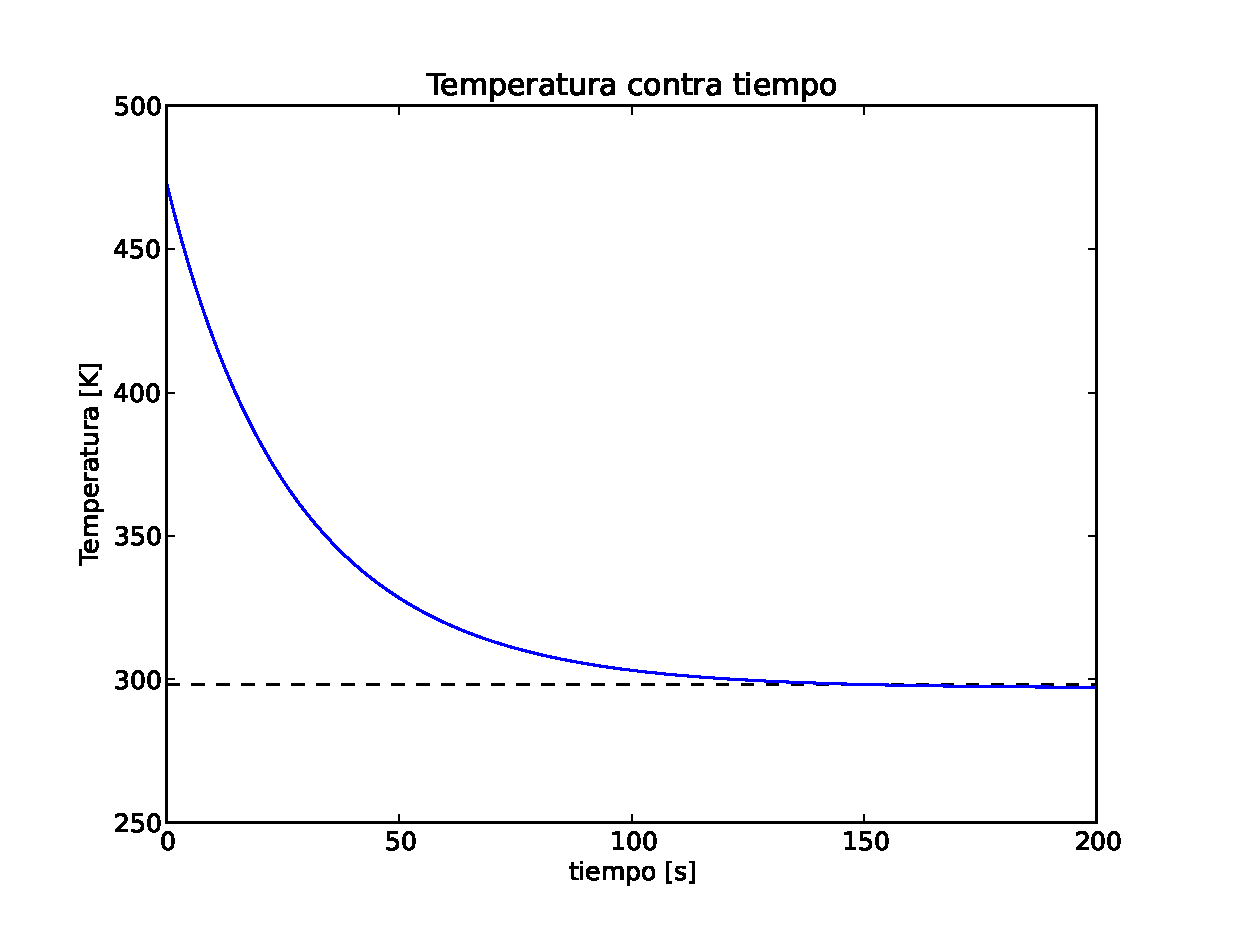
\includegraphics[scale=0.5]{Tema3_2_05_01.eps} 
\end{figure}
\end{frame}
\begin{frame}
\frametitle{Ejercicio adicional}
Con la misma pieza metálica del ejercicio anterior, ahora consideremos que la $T$ inicial es de $25^{\circ}$ y se calienta internamente de forma eléctrica a razón de $q=3000$ W. La ecuación de temperatura es:
\[ \begin{split}
\dfrac{dT}{dt} =& \dfrac{1}{\rho c v} \left[ q - \epsilon \sigma A \left( T^{4} - 298^{4} \right) - h_{c} A \left( T - 298 \right) \right], \\
 T(0) =& 298
 \end{split} \]
Calcular la temperatura de la pieza hasta \textit{t} = minutos, usando RK4, con $h=0.1$ minutos.
\end{frame}
\begin{frame}
\frametitle{Solución gráfica}
\begin{figure}
	\centering
	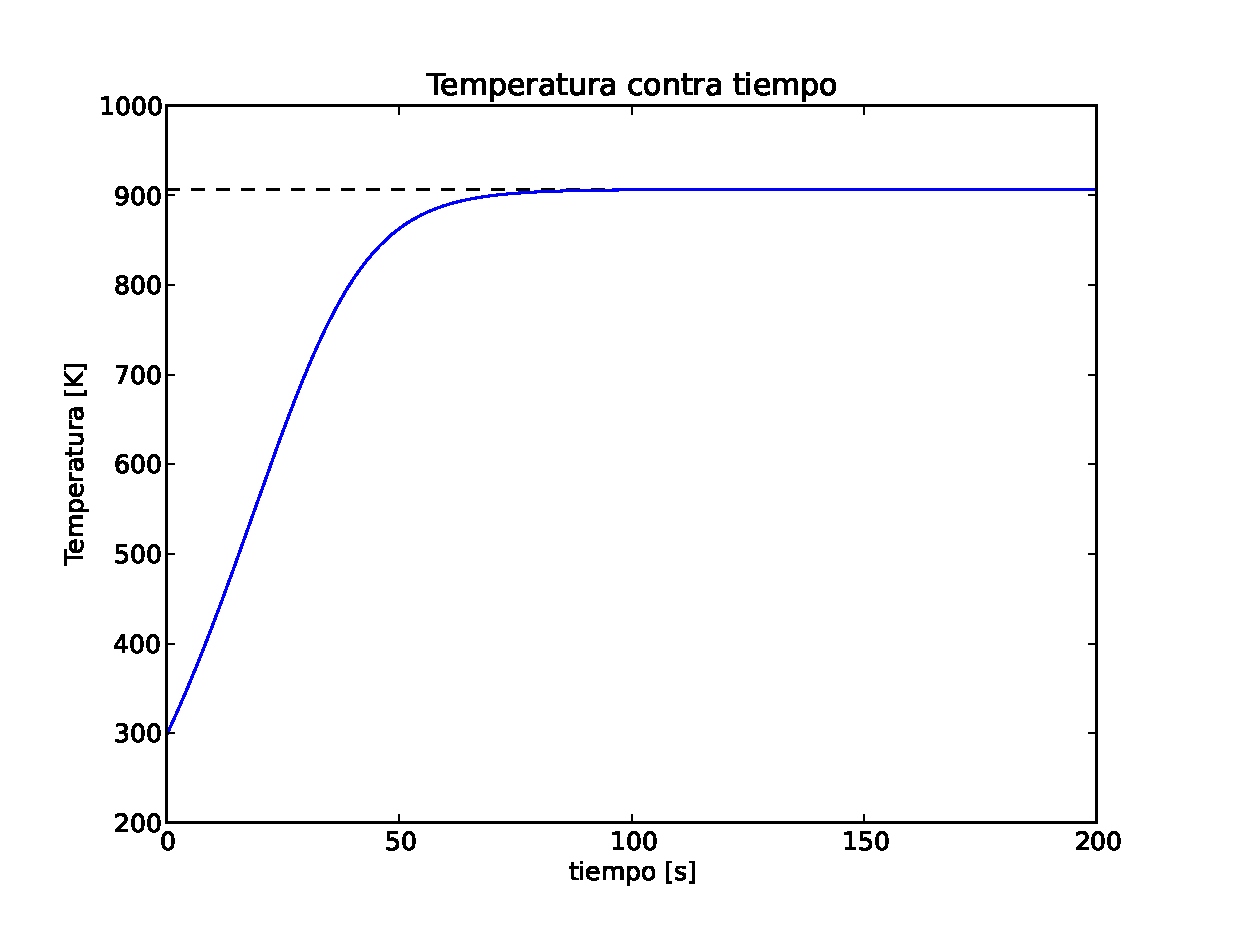
\includegraphics[scale=0.5]{Tema3_2_05_02.eps} 
\end{figure}
\end{frame}
\end{document}